\chapter{Introduction}

\section{Préambule : compilation}

Pour compiler le projet, vous devez avoir installé le framework Qt (nous avons testé sur la version 5.4.1) et vous devez avoir un compilateur C++11 (nous avons testé sur GCC version 4.6.1). Vous pouvez ensuite importer le projet dedans ou compiler dans un terminal sur Linux, comme ceci :
\code{Shell}{bash}
\begin{lstlisting}
QMAKE=`find / -path "*Qt/*gcc*/bin/qmake" -print0 2>/dev/null` # Peut être un peu long
mkdir -p build && cd build/
$QMAKE ../ProjectCalendar/ProjectCalendar.pro -r -spec linux-g++ CONFIG+=debug
make clean && make
\end{lstlisting}

\section{Modélisation}

Après avoir étudié le sujet, nous avons commencé le projet par une étape essentielle de modélisation. Nous avons représenté toutes les classes \og métiers\fg{} dans un schéma UML. Nous avons pour cela réutilisé des \textit{Design Patterns}, tels que \textbf{Singleton} pour les managers (qui sont en fait des \textit{wrappers} de \lstinline{std::vector}). ou \textbf{Composite} (une \lstinline{TacheComposite} contient d'autres \lstinline{Tache}, qui peuvent être de plusieurs types : composite, unitaire ou unitaire et préemptable).

\begin{figure}[h!]
  \centering
    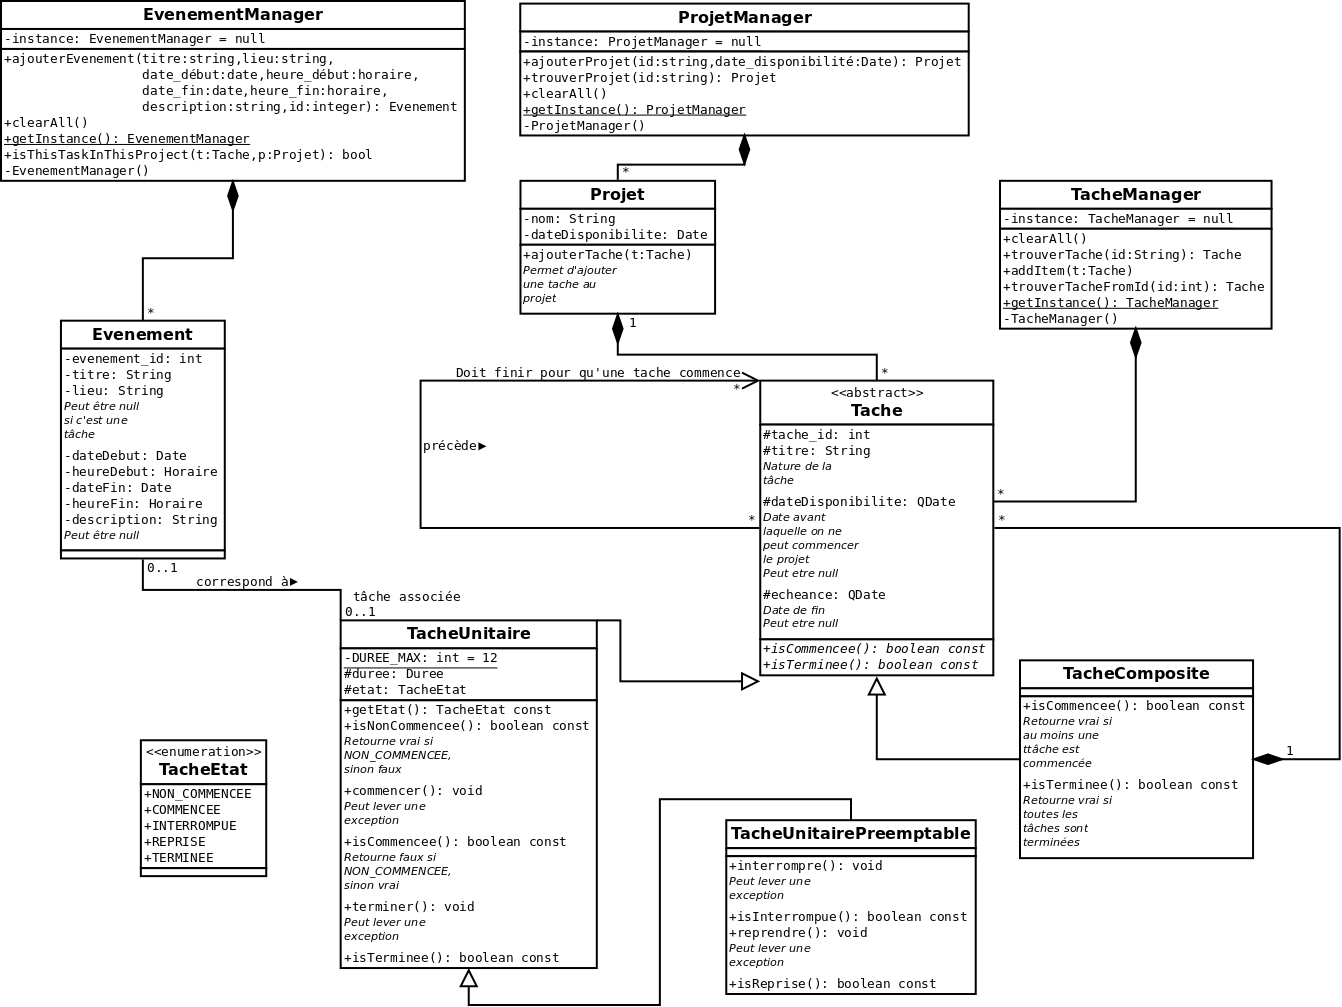
\includegraphics[width=0.8\textwidth]{../modelisation/UML.png}
    \caption{UML des classes métiers}
\end{figure}

\section{Choix techniques}

\subsection{Qt ou STL}

Le \textit{framework} Qt offre de nombreuses classes qui sont des améliorations des classes standards du C++, comme par exemple \lstinline{QString}, qui n'est finalement qu'un \lstinline{sdt::string} amélioré. Ainsi, pour pouvoir plus facilement manipuler les interfaces graphiques, nous avons décidé de n'utiliser que des classes propres à Qt lorsque cela était possible. En voici une liste non exhaustive :
\begin{itemize}
  \item \lstinline{QString}
  \item \lstinline{QTime}
  \item \lstinline{QDate}
  \item \lstinline{QDebug} (pour afficher sur la sortie standard)
  \item ...
\end{itemize}
Seul \lstinline{std::vector} a été utilisé à la place de \lstinline{QVector}, sans raison particulière.

\subsection{Sauvegarde de l'application}
Pour sauvgarder les programmations, projets et tâches de notre application, nous avions le choix entre le XML, le JSON et une base de données SQLite. \textbf{Notre choix s'est porté sur SQLite}. En effet, utiliser un SGBD\footnote{Système de Gestion de Base de Données} offre de nombreux avantages :
\begin{itemize}
  \item Possibilité d'assurer une forte cohérence des données grâce à des contraintes (\textit{check})
  \item Possibilité d'empêcher l'utilisateur de modifier la base de donnée dans un éditeur de texte (cela reste possible en ligne de commande ou avec un logiciel, mais beaucoup moins simple)
  \item Pas de \textit{parsing} à faire comme avec XML et JSON. \textit{Parser} un XML est relativement compliqué à mettre en place (bien qu'il existe des classes pour manipuler le XML), tandis que SQLite est très bien intégré dans Qt, avec des classes pour les requêtes, la gestion d'erreur, etc.
\end{itemize}

\subsection{Interface graphique}

Pour créer l'interface graphique, nous avions le choix entre tout coder \og à la main\fg{} ou utiliser Qt Designer. Après avoir commencé à tout faire à la main, nous nous sommes rendus que la moindre modification ou l'ajout d'un élément graphique entraînait la nécessité de modifier beaucoup de code. \textbf{Nous avons donc finalement décidé d'utiliser Qt Designer}, qui permet de créer des interfaces graphiques facilement et rapidement.

\medskip

Par la suite, nous avons modélisé au papier nos interfaces graphiques, pour nous mettre d'accord et pouvoir par la suite implémenter chacun de notre côté l'interface.